\section{Evaluation}
\label{sec:evaluation}

\begin{figure}[!t]
\centering
 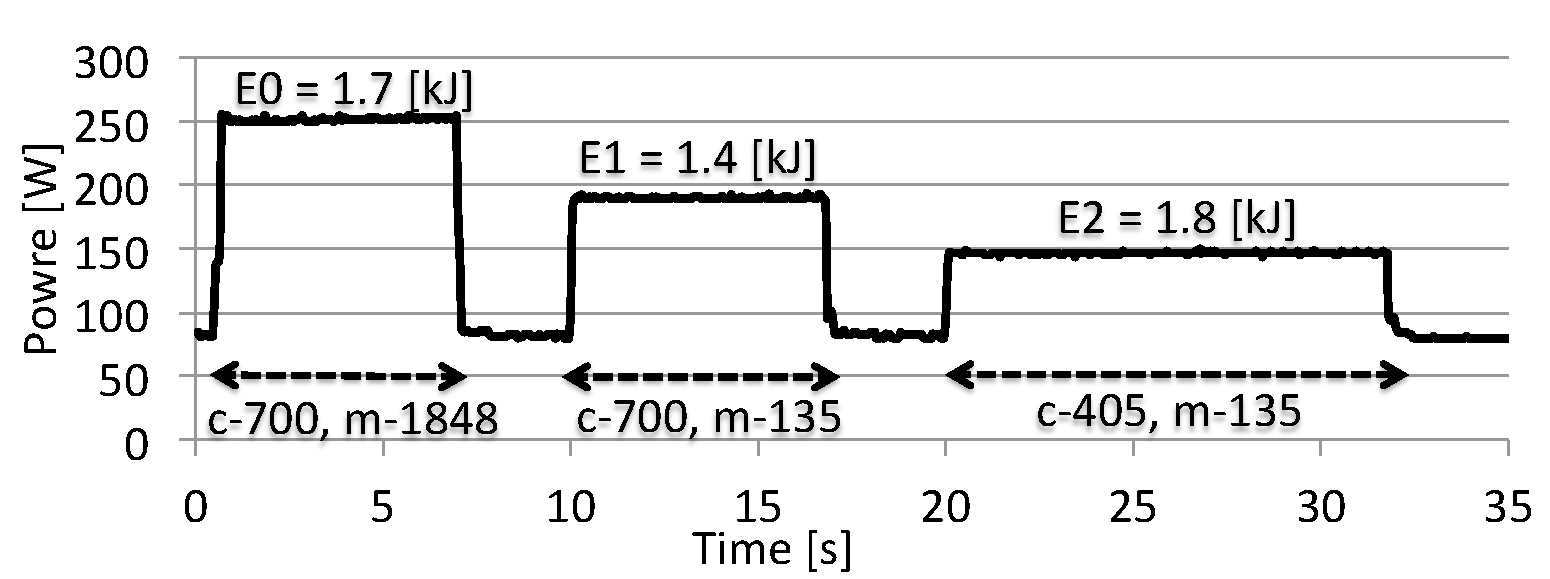
\includegraphics[width=0.45\textwidth]{figures/madd-time-power.pdf}
 \caption{Power consumption and execution time of the $512\times512$
 matrix addition program.}
 \label{fig:madd-time-power}
\end{figure}

We first investigate the impact of GPU core and memory clocks on
GPU-intensive workload executing twenty thousands loops of $512\times512$
matrix addition.
The voltage and frequency of the GPU is changed three times during the
operation, while the CPU is fixed at the minimum level to focus on the
behavior of the GPU.
Figure \ref{fig:madd-time-power} shows the power consumption of the
system in this setup, where ``c-*'' and ``m-*'' stand for the GPU core
and memory clocks respectively, while ``E*'' represents the cummulative
energy consumption of the corresponding duration.
What is learned from this experiment is that energy consumption is
sensitive to the GPU core and memory clocks.
Lowering the memory clock to 135MHz successfully reduces energy
consumption, but the further downscaling of the core clock to 405MHz
counter-increases energy consumption.
This indeed implies DVFS algorithms dominate the power and performance
of GPU-accelerated systems.

We next coordinate the GPU and the CPU using more realistic workload
from the Rodinia benchmark suite.
To simplify the setup, we consider only high (maximum) and low
(minimum) core clocks, meaning that we evaluate four configurations of
(GPU-L, CPU-L), (GPU-H, CPU-L), (GPU-L, CPU-H), and (GPU-H, CPU-H),
where ``*-L'' and ``*-H'' represent the low and high core clocks. 
In an idle state, however, the clocks are always down-scaled to the
minimum level.
We also add another configuration that keeps at the maximum clocks even
though the GPU is idle, in order to see the impact of elementary
coordinated DVFS on GPU-accelerated systems.
Figure~\ref{fig:rodinia-time}~and~\ref{fig:rodinia-energy} respectively
show the execution time and energy consumption of four representative
programs of the Rodinia benchmark suite.
Regarding the execution time, ``all-H'' always takes the shortest
execution time, as it consistently keeps at the maximum performance level.
Other configurations however depend on workload.
For example, the execution time of \texttt{heartwall} -- GPU-intensive
workload -- can be decreased by setting the high GPU clock, whereas that
of \texttt{hotspot} is rather affected by the CPU clock.
The characteristic of energy consumption is more complicated.
For some workload, lowering the clock causes an increase in energy
consumption, as the duration of execution is increased, consuming more
cumulative power consumption.
In other words, GPU-intensive workload should generally use the high GPU
clock so that it completes operation as soon as possible to minimize
energy.
Apparently, ``all-H'' is not a good idea in terms of energy; the clock
should be minimized when the device is not used.
Hence, DVFS is certainly desired but the design of its algorithms is
left an open issue.

\begin{figure}[!t]
\centering
 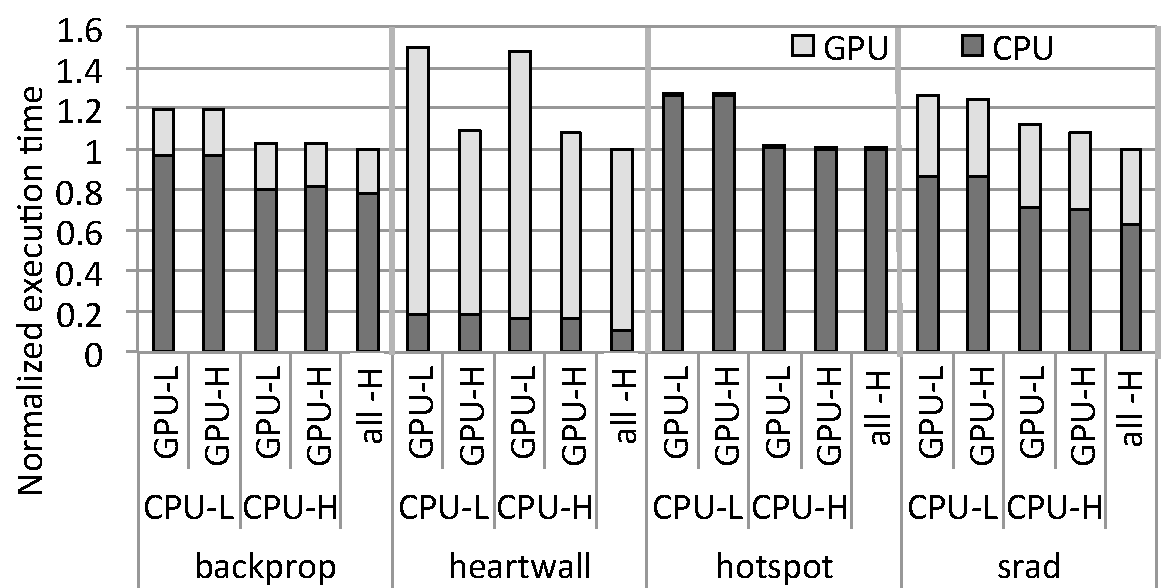
\includegraphics[width=0.45\textwidth]{figures/rodinia-time.pdf}
 \caption{Execution time of the Rodinia programs.}
 \label{fig:rodinia-time}
\end{figure}

\begin{figure}[!t]
\centering
 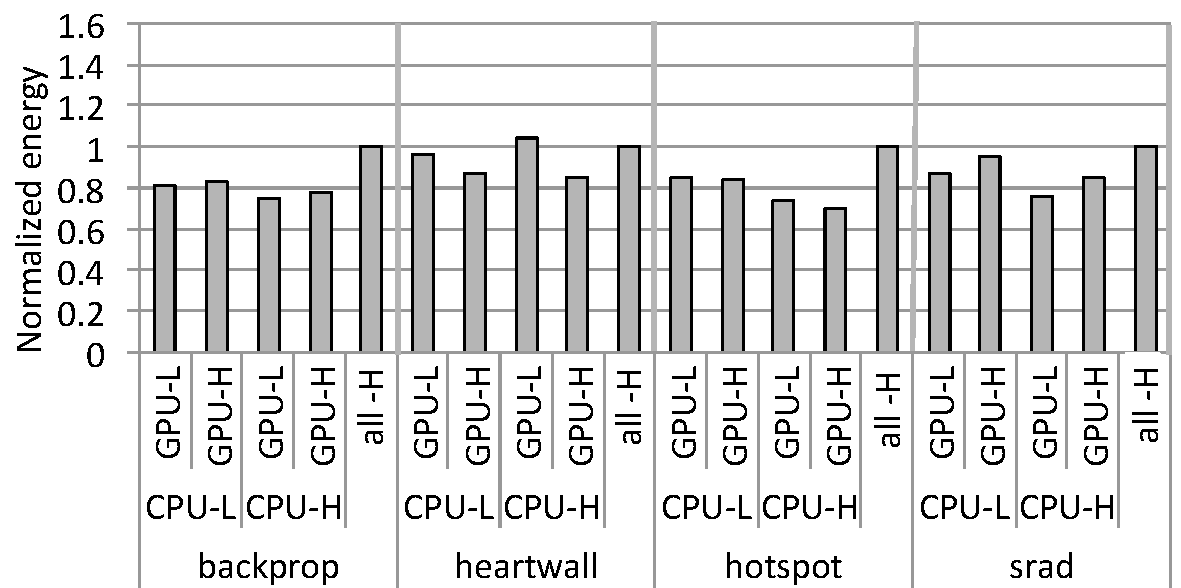
\includegraphics[width=0.45\textwidth]{figures/rodinia-energy.pdf}
 \caption{Energy consumption of the Rodinia programs.}
 \label{fig:rodinia-energy}
\end{figure}

\begin{figure}[!t]
\centering
 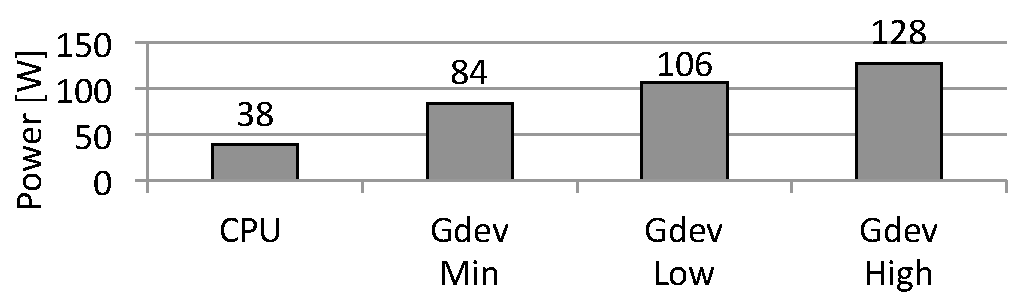
\includegraphics[width=0.45\textwidth]{figures/idol.pdf}
 \caption{Power consumption in an idle state.}
 \label{fig:idle}
\end{figure}

\begin{figure*}[!t]
  \centering
  \subfigure[\texttt{Matrix Addition}]
    {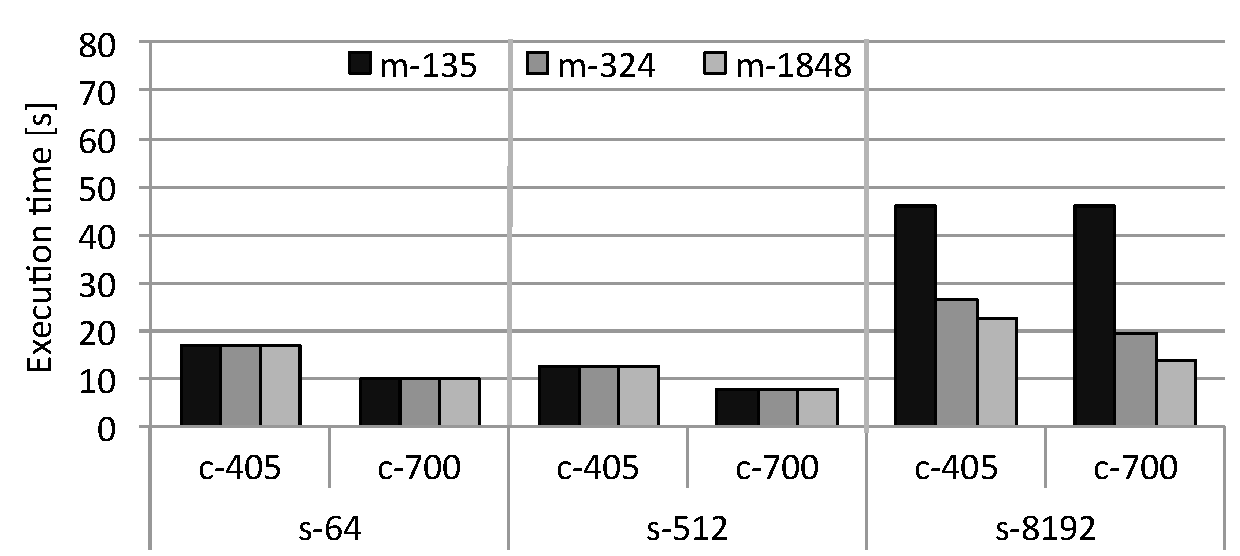
\includegraphics[width=0.45\textwidth]{figures/madd-nvidia-time.pdf}
    \label{madd-time}}
  \subfigure[\texttt{Matrix Multiplication}]
    {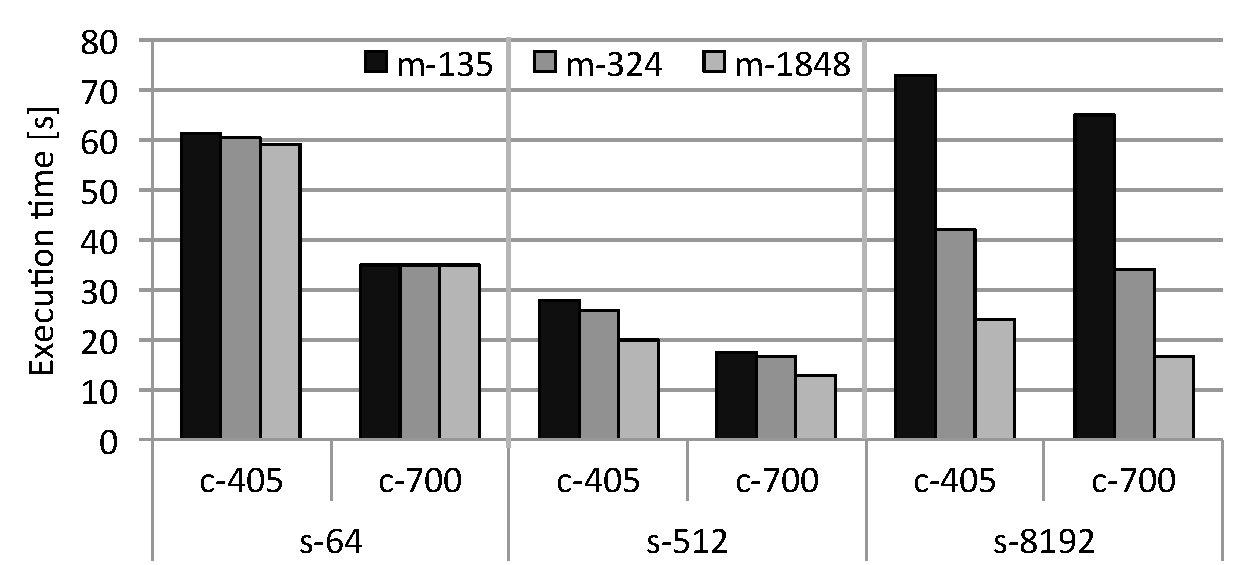
\includegraphics[width=0.45\textwidth]{figures/mmul-nvidia-time.pdf}
    \label{mmul-time}}
  \vspace{-5.0mm}
  \caption{Execution time of the matrix addition and multiplication
 programs.}
  \label{fig:gpu-time}
\end{figure*}

\begin{figure*}[!t]
  \centering
  \subfigure[\texttt{Matrix Addition}]
    {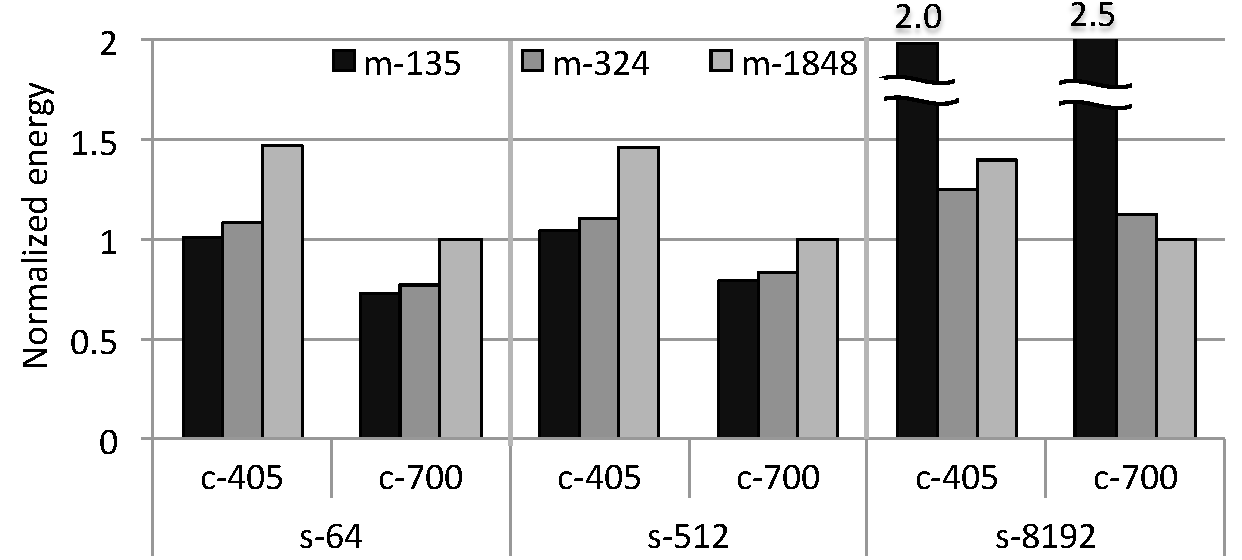
\includegraphics[width=0.45\textwidth]{figures/madd-nvidia-energy.pdf}
    }
  \subfigure[\texttt{Matrix Multiplication}]
    {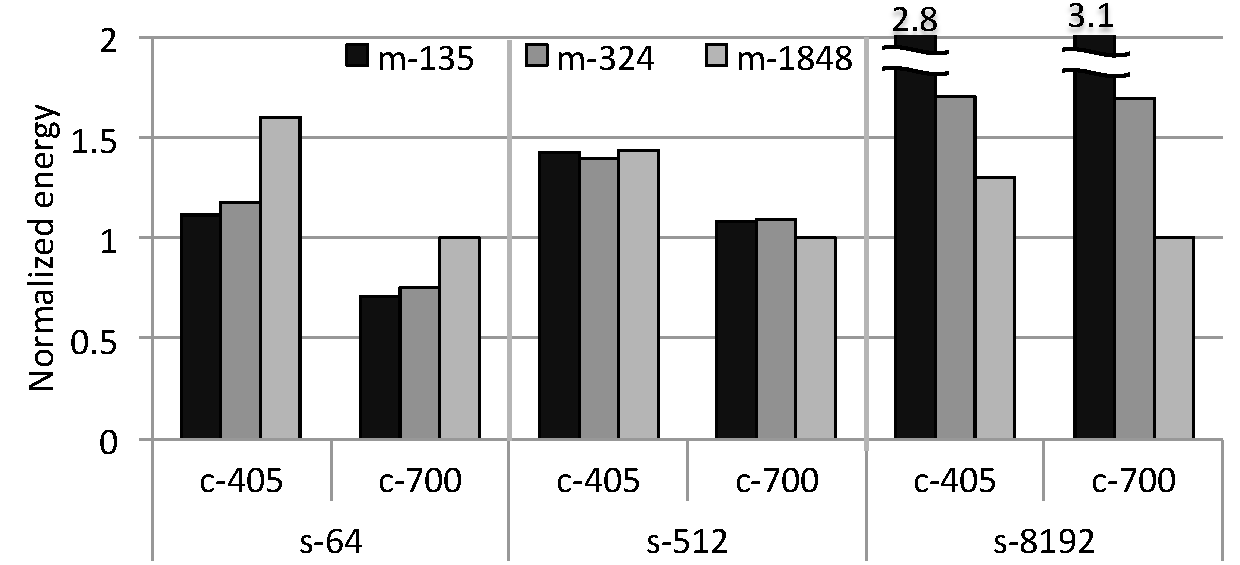
\includegraphics[width=0.45\textwidth]{figures/mmul-nvidia-energy.pdf}
    }
  \vspace{-5.0mm}
  \caption{Energy consumption of the matrix addition and multiplication
 programs.}
  \label{fig:gpu-energy}
\end{figure*}

\begin{figure}[!t]
  \centering
  \subfigure[\texttt{Execution Time}]
    {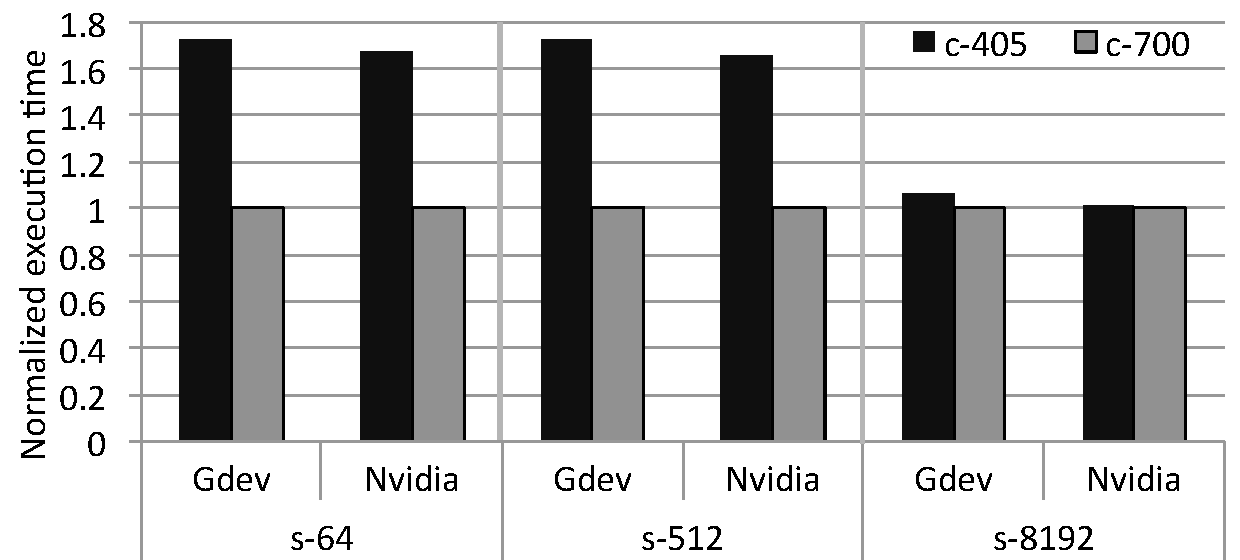
\includegraphics[width=0.45\textwidth]{figures/madd-gdev-nvidia-time.pdf}
    }
  \subfigure[\texttt{Energy Consumption}]
    {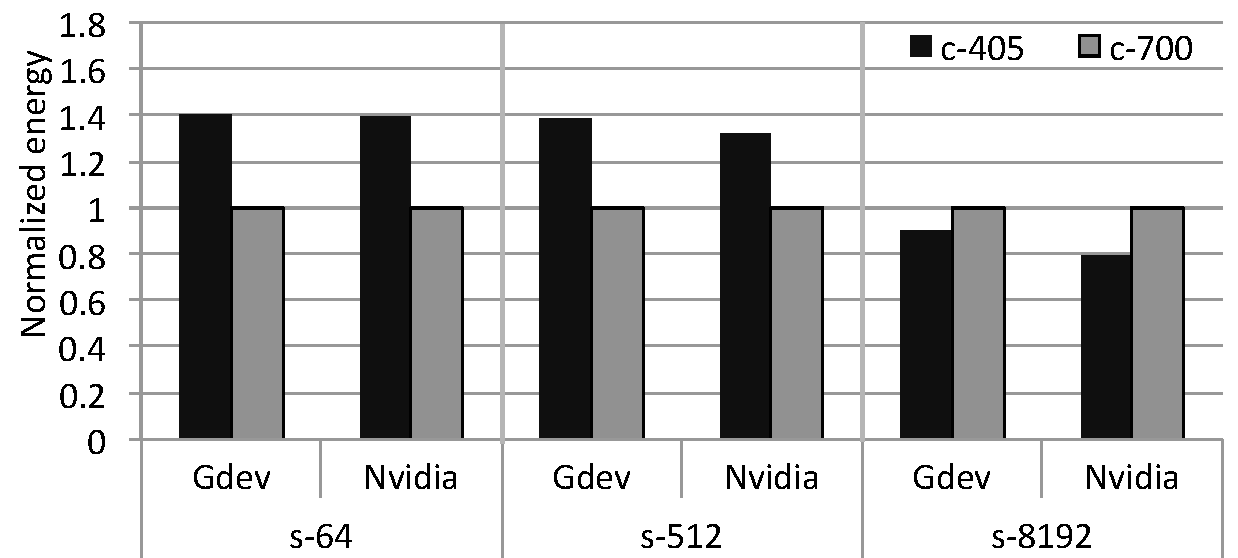
\includegraphics[width=0.45\textwidth]{figures/madd-gdev-nvidia-energy.pdf}
    }
  \vspace{-5.0mm}
  \caption{Comparison of the NVIDIA proprietary and the Gdev open-source
 runtimes and drivers.}
  \label{fig:nvidia-gdev}
\end{figure}

In the above experiments, we have never observed that energy consumption
is reduced by lowering the CPU clock. 
This is because lowering the CPU clock causes the GPU to increase the
duration of an idle state, and there is no power gating support for the
GPU at the moment.
Hence, energy is always wasted when the GPU is idle.
We demonstrate how energy is wasted in an idle state, when (i) the GPU
is not present and (ii) is present with three levels of a set of voltage
and frequency.
Figure~\ref{fig:idle} shows the average power consumption of those four
cases obtained by running the system for 60 seconds.
The CPU consumes no more than 38W on average, whereas the GPU-installed
systems consume a different scale of power depending on the configured
set of voltage and frequency.
This observation encourages the system not to downscale the voltage and
frequency of the CPU, unless the GPU supports power gating to totally
cut off its consuming power.
Another lesson learned from this experiment is that the power
consumption of the GPU is significant even in an idle state, meaning
that DVFS is strongly desired for the GPU with whatever overhead it has
to pay for changing the performance level.

The preceding evaluation indicates that the CPU is a weak factor for
energy savings of GPU-accelerated systems.
Henceforth, we restrict our attention to the GPU.
According to the traditional power modeling~\cite{Hsu2001}, lowering the
core clock is often effective for memory-intensive workload.
Our next evaluation verifies if the same is true for the GPU.
We use matrix addition and multiplication programs with varied sizes of
data.
A small size of data reduces memory accesses, while a large size of data
makes the workload memory-intensive.
Figure~\ref{fig:gpu-time}~and~\ref{fig:gpu-energy} show the execution
time and energy consumption of those matrix computations, where ``s-*''
represents the number of matrix row/column.
A difference between ``s-64'' and ``s-8192'' explains that memory-clock
scaling is more effective for such computations that use a smaller size
of data.
This is because the execution time of such computations is not
affected by lowering the memory clock.
Another observation is that energy cannot be saved by lowering the core
clock, because these matrix computations are consistently
compute-intensive.
If the core clock is downscaled, their execution time is highly
increased, which results in an increase in cumulative power
consumption.

Seen from the above experiments, system energy could be reduced
by about 28\% retaining a decrease in performance within 1\%.
These experimental results encourage that DVFS algorithms for
GPU-accelerated systems should be weighted on the GPU rather the CPU,
though their energy optimization is very challenging, given many factors
of design knobs including CPU/GPU, core/memory, and workload
characteristics.

Finally, we compare NVIDIA's proprietary software and Gdev.
This is an important and practical investigation in that NVIDIA's
proprietary software does not expose a system interface to change
the voltage and frequency of the GPU dynamically at runtime, and hence
the development of DVFS algorithms in future work will inevitably depend
on Gdev.
The basic performance of Gdev is competitive to NVIDIA's proprietary
software~\cite{Kato2012}, but we have to evince that Gdev is also
reliable for power management.
The test program exploits matrix addition with varied sizes of data.
Figure~\ref{fig:nvidia-gdev} shows the execution time and energy
consumption of the matrix addition programs using different scales of
GPU core clocks, where the GPU memory clock is fixed at 135MHz.
In this experiment, ``s-8192'' benefits from lowering the core clock,
because the workload is memory-bound due to a large size of matrix, and
the execution time is not much affected by the core clock, while every
is effectively saved.
The most remarkable observation is that NVIDIA's proprietary software
and Gdev exhibit almost the same results on the execution time and energy
consumption.
This implies that the result of our on-going research using Gdev could
be easily propagated to the real product, once energy management
interfaces are employed by vendor's software.
